\documentclass[10pt, a4paper, oneside]{ctexart}
\usepackage{amsmath, amsthm, amssymb, graphicx}
\usepackage[UTF8]{ctex}
\usepackage[bookmarks=true, colorlinks, citecolor=blue, linkcolor=black, unicode]{hyperref}
\usepackage{soul} % 导入 soul 包
\usepackage{color} % 颜色包,color 必须导入,xcolor 建议导入
\usepackage[svgnames]{xcolor}
\graphicspath{{./image}}
\usepackage{geometry}
\geometry{left=2.54cm, right=2.54cm, top=3.18cm, bottom=3.18cm}\usepackage{blindtext}
\parindent=0pt

% 导言区
\title{\LaTeX 高等数学上下册笔记}
\author{XBY}
\date{\today}

\begin{document}
\begin{sloppypar}
	\maketitle
	\setcounter{tocdepth}{4}
	\tableofcontents
	\pagenumbering{Roman}
	\setcounter{page}{0}

	\def\oiint{{\bigcirc}\kern-11.5pt{\int}\kern-6.5pt{\int}}
	\def\oiiint{{\bigcirc}\kern-12.3pt{\int}\kern-7pt{\int}\kern-7pt{\int}}

	\newpage
	\section{上册}
	无穷小量$(\lim=0)$无穷大量(绝对值无限变大).
	$\sqrt{n}$是$n\to+\infty$时无穷大量.
	收敛即有界、极限唯一,有界不收敛.\\
	四则运算(极限分母不为0)前提$\lim a_n$存在.
	常数可提,指数可移出内外.\\
	等比级数公比q.|q|<1收敛于$\frac{a}{1-q}$否则发散.

	\subsubsection{级数性质}
	两个收敛级数可以逐项相加减.
	去掉、加上、改变有限项不影响敛散性.
	级数收敛,一般项趋近于0,一般项趋向0不一定级数收敛(调和级数).
	调和级数:$\sum_{n - 1}^{\infty}\frac{1}{n}$
	P-级数 $\sum_{n - 1}^{\infty}\frac{1}{n^p}\space p>1$收敛\\
	比较判别法:
	正向数列敛散性,$u_n\Leftarrow v_n$ 均为正项级数,$v_n$收敛,$u_n$收敛;$u_n$发散$v_n$发散
	$\lim f(x) = A \Leftrightarrow f(x) = A + a,\lim a = 0$.a无穷小量 A极限值.
	常数/无穷小量间乘积代数和=无穷小量.
	有界函数$\times$无穷小量.
	无限、变大 $\to$无穷大量.
	无穷小量的比较为收敛速度快慢.
	\begin{gather*}
		a=o(b)\quad
		\lim \frac{a}{b}=\begin{cases}
			0(\text{a是比b高阶无穷小}) \\
			C(\neq 1)                  \\
			1 \Rightarrow a \sim b(\text{等价})
		\end{cases}\quad
		X\to 0,|x| << 1
		\begin{cases}
			\ln(1+x)=x                                \\
			e^x = x + 1                               \\
			(1+x)^{\frac{1}{n}} = a + \frac{1}{n} * x \\
			\tan x = \sin x = x;                      \\
			1-\cos x = \frac{1}{2}x^2
		\end{cases}
	\end{gather*}
	\begin{align*}
		\text{y=f(x)在x0处连续} & \Leftrightarrow \lim_{\Delta x\to0}\Delta y=0 \\
		                        & \Leftrightarrow \lim_{x\to x_0}f(x)=f(x_0)
	\end{align*}

	初等函数在定义域内处处连续.连续性:函数值等于极限.
	\subsubsection{间断点}
	一类 点左右极限均存在 可去间断点(极限相等),跳跃间断点(不相等)
	二类 左右至少一个极限不存在 无穷间断点(极限无穷) 振荡间断点(趋近时在两值变动)
	连续函数的四则运算/反函数/复合函数仍是
	求导增量比的极限
	导数定义\\
	求增量、算比值、取极限
	左右导数均存在且相等$\Leftrightarrow$fx在x0可导(分段函数)
	角点/尖点处导数不存在
	连续$\Rightarrow$可导
	不可导情况:无定义、不连续、不光滑、导数值$\infty$

	反函数导数等于原函数倒数

	幂指函数求导
	1.写成e的指数形式
	2.等式两边同取ln

	隐函数求导
	F(x,y) = 0
	尝试隐函数化显函数
	实际:从方程出发求导,设函数y = y(x),等式两边同时求导
	参数式函数求导方法
	结论:因变量、自变量对参数(中间变量)求导之商
	$$
		\begin{cases}
			1.\text{隐函数化显函数再求导}                        \\
			2.\text{隐函数左右对x求导 y=f(x)}                    \\
			3.\text{利用1阶微分形式不变性分别对y,x求导,移项求导} \\
			4.\text{n元隐函数看作(n+1)元函数,在多元函数偏导数之商求导}
		\end{cases}
	$$
	$$
		[u(x)\pm v(x)]^{(n)}=u^{(n)}(x)\pm v^{(n)}(x) \quad [Cu(x)]^{(n)}=Cu^{(n)}(x)$$
	莱布尼茨公式
	$$
		[u(x)\cdot v(x)]^{(n)}=\sum_{k=0}^{n}C_n^k u^{(n-k)}(x)v^{(k)}(x)
	$$

	\subsection{特殊高阶导数}
	\begin{align*}
		 & (\sin x)^{(n)}==\sin(x+\frac{n\pi}{2})
		 & (\cos x)^{(n)}=\cos(x+\frac{n\pi}{2})                                                            \\
		 & (\ln x)^{(n)}=(-1)^{(n-1)}\frac{(n-1)!}{x^n} & (\ln(1+x))^{(n)}=(-1)^{n-1}\frac{(n-1)!}{(1+x)^n} \\
		 & (\frac{1}{x})^{(n)}=(-1)^n\frac{n!}{x^{n+1}}
	\end{align*}
	$$\Delta y = A\cdot\Delta x + o(\Delta x)$$
	$o(\Delta x)\Delta x$高阶无穷小 $\Delta x$常数 称呼y在$x_0$处可微
	$dy = A\times\Delta x $可微$\Leftrightarrow$可导
	=>$x_0$连续
	$A = f^{\prime}(x_0)$
	$$d(uv) = (vdu + udv)\quad d(\frac{u}{v}) =\frac{vdu - udv}{v^2}$$
	复合函数
	$u = \varphi(x) y=f(u)$
	$dy = f^{\prime}(u)du$微分形式不变性
	估算函数在某点函数值 $f(x_0 + \Delta x) = f(x_0)  + f^{\prime}(x)\Delta x$
	\vspace*{1\baselineskip} \\
	微分中值定理 函数在区间整体性质与该区间某以点处的导数之间关系(微分基本定理)
	极值 局部相对
	费马定理:x0处可导 x0极值点 $f^{\prime}(x0) = 0$(x0驻点)
	[a,b]连续可导
	罗尔定理:f(a)=f(b) 至少存在一个驻点
	拉格朗日中值定理:至少存在一点t $\frac{f(b)-f(a)}{b-a} = f^{\prime}(t_0)$
	导数为0$\Leftrightarrow$函数为常函数

	f(x),g(x)均可导极限同时均为0或$\lim_{\infty}\frac{f^{\prime}(x)}{g^{\prime}(x)}$存在或=$\lim_{\infty}\frac{f(x)}{g(x)} = \lim_{\infty}\frac{f^{\prime}(x)}{g^{\prime}(x)}$\par
	$0 \times \infty = \frac{0}{ \frac{1}{\infty}} , \frac{\infty}{\frac{1}{0}},
		\infty \times \infty $"合二为一"$0^0,1^\infty,\infty^0$用
	$$
		\begin{cases}
			a=e^{\ln a}                                        \\
			b\ln a = \ln{a^b}                                  \\
			f(x)^g(x) = e^{\ln{f(x)^g(x)}} = e^{g(x)\ln{f(x)}} \\
			g(x)\ln{f(x)}
		\end{cases}=0\times\infty
	$$

	极值点增减区间交界点
	求极值点:
	1驻点、不可导点
	2确定单调区间
	3交界点函数值

	1驻点(一阶导数为0),此点二阶导数不为0则为极值点 >0极小值 <0极大值

	最大(小)值可能在区间内部的驻点、不可导的点及区间的端点处取得.
	凸凹性$f^{\prime\prime}(x)>0(f^{\prime}(x)$递减)凹性 凸凹交界 拐点 且二阶导存在=>$f^{\prime\prime}(x0) = 0$
	水平渐进线、铅直渐进线

	原函数存在定理 f(x)在区间I连续 必有原函数F(x)在I上
	被积函数常数可移外
	不定积分线性性质
	\begin{align*}
		 & sec^2 x = 1 + tan^2 x                                  &                                                            \\
		 & \int\frac{dx}{1+x^2}=\arctan x + C=-arccot x + C \quad & \int\frac{dx}{\sqrt{1-x^2}}=\arcsin x + C = -\arccos x + C \\
		 & \sec x\tan xdx=\sec x + C\quad                         & \csc x\cot xdx=-\csc x + C
	\end{align*}

	第一类/第二类换元法
	一:积分形式不变性  凑微分法
	\begin{gather*}
		\int f(x)dx=F(x)+C\\
		u=\varphi(x)\\
		\int f(u)du=F(u)+C
	\end{gather*}

	真分式 分子的最高次数低于分母的最高次数, 无公因式可拆为多项分式相加。
	当被积函数为有理假分式时,先将其转化为多项式与真分式的代数和.
	若分子恰是分母的导数
	$$\int \frac{f^{\prime}(x)}{f(x)}dx=\int\frac{df(x)}{f(x)}=\ln f(x)+C$$

	二:
	注意:第二换元法引入了新的变量进行积分,其积分结果中必须回代原变量.
	说明:
	(1)第二换元法主要用于去掉被积函数中的根号但有时并非必用不可.
	(2)被积函数不含根号时,有时也可用第二换元法,作变量代换,引入新变量来简化运算.\\
	一般地,被积函数含有根式(根号内为一次函数)时,可作变量代换.
	$\sqrt[n]{ax+b}=t$
	一般地,被积函数含有根式且根式内是二次函数时,可作三角换元.例如$\sqrt{a^2 - x^2},\sqrt{a^2 + x^2},\sqrt{x^2 - a^2}$

	分别可作代换$x=a\sin t,x=a\tan t,x=a\sec t$消去根式.用三角换元求出原函数后,利用辅助直角三角形来回代原变量比较方便.
	倒代换:令$x=\frac{1}{t}$
	分步积分法
	公式:
	\begin{gather*}
		\text{交换了原式中uv位置}\\
		\int \colorbox{green}{u}d\colorbox{yellow}{v}=uv-\int \colorbox{yellow}{v}d\colorbox{green}{u}
	\end{gather*}

	选取两个原则:
	\begin{center}
		(1)dv较容易凑出;\\
		(2)$\int vdu$要比$\int udv$容易求出.
	\end{center}

	如果被积函数是幂函数与反三角函数乘积或幂函数与对数函数的乘积,就可以考虑用分部积分法求不定积分,并且令反三角函数或对数函数为u.
	如果被积函数是指数函数和正弦(或余弦)函数的乘积,考虑用分部积分法.经过两次分部积分后会出现原来的积分,通过合并同类项即可求得不定积分.
	\vspace*{1\baselineskip} \\
	微分方程 含未知函数导数/微分  函数一元常微分方程 函数最高阶导数为微分方程的阶
	特解通解(含C)
	1.可分离变量
	从通解中确定出特解的条件称为初始条件(初值条件)$\to$初值问题
	一阶线性微分方程:未知函数及其导数都是一次的.
	$$\frac{dy}{dx}+P(x)y=Q(x)$$
	通解:$y=e^{-\int P(x)dx}[\int Q(x)e^{\int P(x)dx}dx+C]$

	Q(x) = 0齐次(移项分离变量)否则非齐次
	通解

	$$e^(aln(b)) = b^a$$

	定积分
	(交换定积分的上下限,积分值变号)
	a=b时定积分为0

	积分区间可加性 c任意
	定积分的估值定理

	中值定理

	右侧被称作函数f(x)在[a.b]上平均值
	定积分换元
	换元必须相应换限.
	换元后新运算不必代回原变量
	区间对称$\to$奇函数偶函数

	周期:$\int_{a}^{a+T}f(x)dx=\int_{0}^{T}f(x)dx$
	恒等式:$$
		\int_{0}^{\pi /2}sin^nxdx=\int_{0}^{\pi / 2}cos^nxdx=\begin{cases}
			\frac{n-1}{n}\cdot\frac{n-3}{n-2}\cdots\frac{3}{4}\cdot\frac{1}{2}\cdot\frac{\pi}{2}\cdot n为正偶数 \\
			\frac{n-1}{n}\cdot\frac{n-3}{n-2}\cdots\frac{4}{5}\cdot\frac{2}{3} n为大于1正奇数
		\end{cases}$$
	反常积分广义积分 性质:积分区间无穷,被积函数区间无界
	$$
		\int_{a}^{+\infty}f(x)dx=\lim_{b \to \infty} f(x)dx(a<b)\begin{cases}
			=C 收敛 \\
			\ne C 发散
		\end{cases}
	$$
	$$
		\int_{-\infty}^{+\infty}f(x)dx=\int_{-\infty}^{c}f(x)dx + \int_{c}^{+\infty}f(x)dx\begin{cases}
			=C 收敛 \\
			\ne C 发散
		\end{cases}
	$$

	\subsection{二阶三阶行列式}
	上三角、下三角和对角行列式的值都是其主对角线上的元素之积.
	克莱姆法则
	\begin{center}
		1.方程组中未知量的个数等于方程的个数;
		2.系数行列式不为零.
	\end{center}
	常数项全为0齐次线性
	一般:D=0无解或至少有一解
	齐次D!=0只有零解
	转置矩阵左下翻右上
	行列式经过转置仍相等
	同一行列可提公因式至行列式前
	某一行一列为0 行列式0
	互换两行/列,行列式变号
	两列/行成比例 = 0
	一行/列同乘一数加至另一行/列对应,不变
	行列展开.
	代数余子式:$A_ij=(-1)^(i + j)M_ij$
	n阶行列式的值等于它的任意一行(列)的元素与其对应的代数余子式的乘积的和.
	增广矩阵
	行阶梯、行最简(线性方程组的解)
	系数行列式判断方程组是否有解
	消元法解线性方程组具体方法是:对线性方程组的增广矩阵进行初等行变换,转化为行最简矩阵,由行最简矩阵可以方便地求出原方程组的解.
	矩阵运算
	结合律
	左右分配律
	(LambdaA)B=lambda(AB)=A(lambdaB)
	方阵A可逆<=>|A|!=0<=>A为非奇异矩阵

	行列式为零的方阵称为奇异矩阵

	伴随矩阵:行列式A中元素$a_ij$的代数余子式$A_ij$构成的矩阵$A^*$
	$$
		AA^*=|A|E=\begin{bmatrix}
			|A| &     &        &     \\
			    & |A| &        &     \\
			    &     & \ddots &     \\
			    &     &        & |A| \\
		\end{bmatrix}
		A^(-1) = \frac{1}{|A|}A^*
	$$
	\section{下册}
	点P存在邻域U(P)属于E P为E哪点
	点集E的点都是内点,E开集
	P任意邻域内部分属于E,称P边界点
	E全体边界点 E的边界
	开集D内任意两点用属于D的折线连接,称开集D连通
	(开区域)
	闭区域$eg:{(x,y)|1<=x^2 + y^2<=4}$
	点集E,存在实数k,使一切点P属于E与某一定点A距离不超过K,E有界点集,否则无界点集

	P任何邻域内总有无穷点属于E,P是E聚点
	E的边界点可能是E的聚点;
	E的聚点可能是E中的一点

	多元函数极限
	全面极限二重极限
	点趋近点的路径多样
	几条特殊路径趋近点时,即使f(x,y)无限趋近某个确定常数A也不能说极限存在
	两条不同路径趋近,得出不同f值,可以断定二重极限不存在
	二重极限不存在判断:设法选择xoy面上过($x_0, y_0$)的两条曲线y=$\phi_1(x)$与$y=\phi_2(x)$使$\lim_{\substack{x \to x_0\\y=\phi_1(x)}}f(x,y)$与$\lim_{\substack{x \to x_0\\y=\phi_2(x)}}f(x,y)$值不相等
	取路径$\to$建立多元函数关系$\to$化简回一元函数
	最大值最小值定理、介值定理
	一切多元初等函数在其定义区域内是连续的。
	连通点集构成区域
	任何邻域都是区域

	求$\lim_{P \to P_0}f(P)$,若f(P)是初等函数且$P_0$是定义域内点,则f(P)在$P_0$处连续于是$\lim_{P \to P_0}f(P)=f(P_0)$
	连续性$\to$考虑n元初等函数趋近此点n重极限是否等于函数值

	偏导数
	定义:
	函数在点$(x_0,y_0)$的某一邻域内有定义,y固定在$y_0$,x在$x_0$处有增量$\Delta x$,有增量$f(x_0+\Delta x,y_0)-f(x_0,y_0)$极限$\lim_{\Delta x \to 0}\frac{f(x_0 + \Delta x, y_0)-f(x_0,y_0)}{\Delta x}$称为函数z在点(x0,y0)对x的偏导数
	求函数在点偏导数
	解法1:
	分别对自变量求偏导数值
	解法2:
	分别将其他自变量对应值代入原函数得新函数,用剩下一个自变量代入新函数计算。
	偏导数的记号应看作一个整体性的符号(不能看成商的形式)区别于一元函数$\frac{dx}{dy}$

	此例表明,二元函数在一点不连续,但其偏导数却存在.\\
	一元函数在某点可导,则函数在该点一定连续;若函数在某点不连续,则函数在该点一定不可导.二元不同.
	$f_x(x_0, y_0)、f_y(x_0, y_0)$仅仅是函数沿两个特殊方向(平行于x轴、y轴)的变化率,连续即以任何方式趋近于点时函数值趋近$f(x_0,y_0)$,反应函数在此点"全面"状态$\to$二元函数在某点偏导数与函数在该点的连续性之间没有联系。\\
	\begin{figure}[htbp]
		\centering
		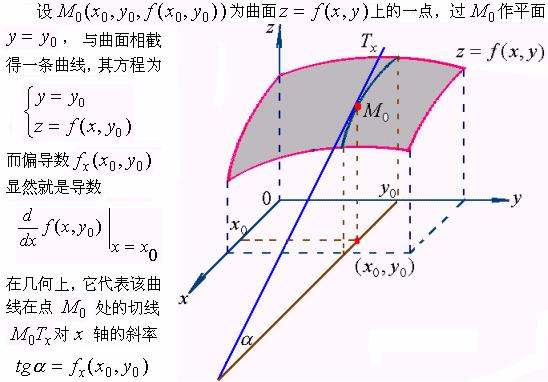
\includegraphics[width=8cm]{image126.jpg}
		\caption{二阶导数空间几何关系}
	\end{figure}
	公式对称、轮换性可简化不同自变量偏导数讨论
	\subsection{高阶偏导数}
	$f_{xy}(x,y),f_{yx}(x,y)$为二阶混合偏导数\\
	简洁记法:
	\begin{align}
		 & \frac{\vartheta^2 z}{\vartheta x^2}=f_{11}(x,y) \\ &\frac{\vartheta^2 z}{\vartheta x\vartheta y }=f_{12}(x,y)
	\end{align}
	定理:如果$z=f(x,y)$的两个二阶混合偏导数$\frac{\vartheta^2 z}{\vartheta x\vartheta y},\frac{\vartheta^2 z}{\vartheta y\vartheta x}$在区域内连续,则未在该区域内这两个二阶混合偏导数必相等
	\colorbox{green}{存在二阶混合偏导数连续的条件下,与求导次序无关}\\
	tip:f(x,y)=0时用$\lim_{x\to 0}\frac{f(x,y_0)-f(x_0,y_0)}{x}求f_x(x_0,y_0)$
	一阶偏导数当作原函数求二阶偏导数\\
	拉普拉斯方程:
	$\frac{\vartheta^2u}{\vartheta x^2}+\frac{\vartheta^2u}{\vartheta y^2}+\frac{\vartheta^2u}{\vartheta z^2}=0$

	$$f(x+\Delta x,y)-f(x,y)\approx f_X(x,y)\cdot \Delta x$$
	偏增量,偏微分
	全增量:多元函数各个自变量都取增量时,因变量获得的增量$\Delta z=f_x(x,y)\Delta x + f_y(x,y)\Delta y + \varepsilon_1 \Delta x + \varepsilon_2 \Delta y$其中$\lim_{\Delta y \to 0}\varepsilon_2 = 0,\lim_{\Delta x \to 0}\varepsilon_1 = 0$\\
	若$$\Delta z = A\cdot\Delta x + B \cdot \Delta y +o(\rho)$$ A,B不依赖于$\Delta x,\Delta y$仅与x,y有关,$\rho=\sqrt{\Delta x^2 + \Delta y^2}$,称函数f(x,y)在点(x,y)处可微分.
	$o(\rho)\to0$时$\Delta z = A\cdot\Delta x + B \cdot \Delta y$称为函数f在(x,y)处的全微分
	\subsection{函数可微分条件}
	偏增量,偏微分

	定理一(必要条件)\\
	函数z在(x,y)处可微分$\Rightarrow (x,y)$偏导数$\frac{\vartheta z}{\vartheta x},\frac{\vartheta z}{\vartheta y}$必定存在全微分,记作$\Delta z = \frac{\vartheta z}{\vartheta x}\cdot\Delta x + \frac{\vartheta z}{\vartheta y} \cdot \Delta y$

	定理二(充分条件)\\
	函数z,$\frac{\vartheta z}{\vartheta x},\frac{\vartheta z}{\vartheta y}$在点(x,y)连续$\rightarrow$该点可微分.
	可微分$\rightarrow$在点连续$\space$注意:$\Delta x \to 0,\Delta y \to 0$等价$\rho = \sqrt{\Delta x^2 + \Delta y^2}\to 0$.\par
	可微分$\rightarrow$偏导数必存在但不一定连续\\
	结论:\begin{center}
		1.偏导数连续$\rightarrow$函数可微分\\
		2.偏导数连续$\nleftarrow$函数可微分
	\end{center}
	二元函数的全微分等于它的两个偏微分之和,即(4)式称之为二元函数微分的叠加原理.
	\begin{figure}[htbp]
		\centering
		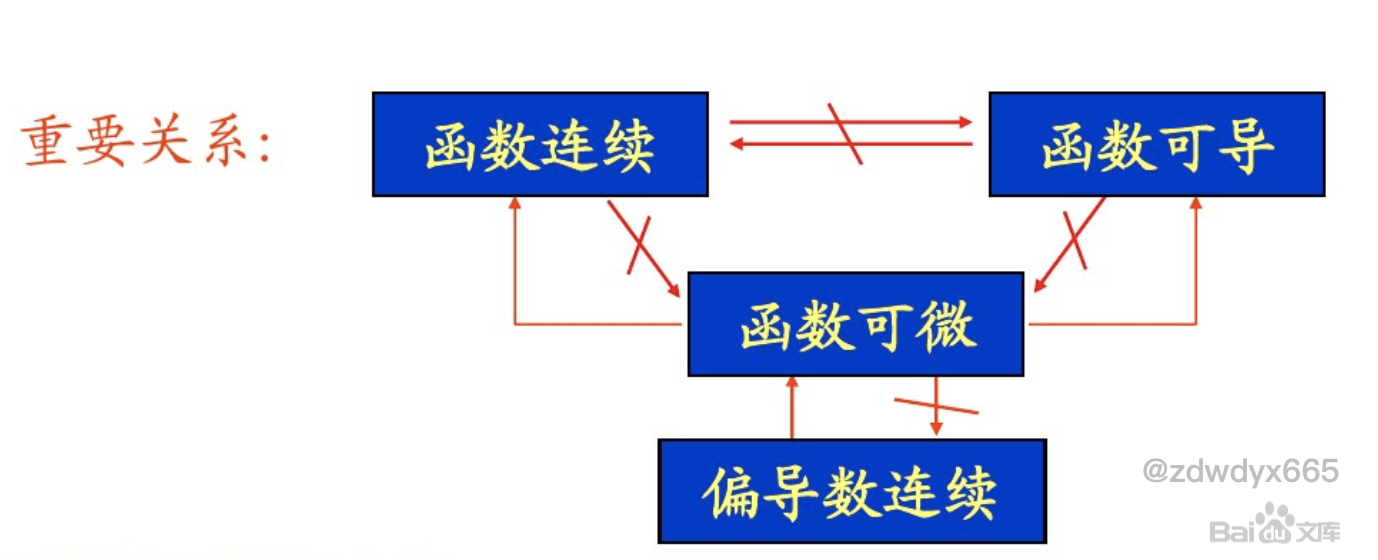
\includegraphics[width=8cm]{image1.png}
		\caption{关系}
	\end{figure}

	\subsection{多元函数求导法则}
	定理:若$u=\varphi(t)$及$v=\phi(t)$在t点可导;函数z=f(u,v)在点(u,v)具有连续偏导数
	复合函数$z=f[\varphi(t),\phi(t)]$在t点可导,导数为:
	$$\frac{dz}{dt}=\frac{\vartheta
			z}{\vartheta u}\cdot\frac{du}{dt}+\frac{\vartheta z}{\vartheta v}\cdot\frac{dv}{dt}$$
	同样方式可推广到中间变量多余两个的情况$z=f(u,v,w),u = \varphi(t), \phi(t), w=\omega(t)$
	\setcounter{equation}{0}
	\begin{equation}\label{全导数1}
		\frac{dz}{dt}=\frac{\vartheta
			z}{\vartheta u}\cdot\frac{du}{dt}+\frac{\vartheta z}{\vartheta v}\cdot\frac{dv}{dt}+\frac{\vartheta
			z}{\vartheta \omega}\cdot\frac{d\omega}{dt}
	\end{equation}
	中间变量不是一元函数而是多元函数
	\begin{equation}\label{全导数2}
		\frac{dz}{dt}=\frac{\vartheta
			z}{\vartheta u}\cdot\frac{du}{dt}+\frac{\vartheta z}{\vartheta v}\cdot\frac{dv}{dt}+\frac{\vartheta
			z}{\vartheta \omega}\cdot\frac{d\omega}{dt}
	\end{equation}
	\subsubsection{全导数}
	\eqref{全导数1},\eqref{全导数2}称作全导数
	\subsection{多元复合函数求导法则}
	\begin{figure}[htbp]
		\centering
		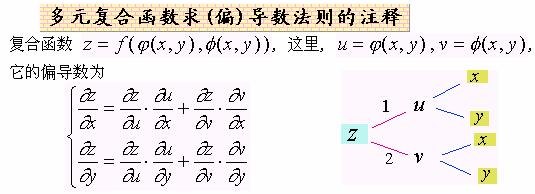
\includegraphics[width=8cm]{image120.jpg}
		\caption{求导法则注释}
	\end{figure}
	锁链法则\\
	连线相乘分线相加
	\subsubsection{隐函数求导}
	二元方程F(x,y)可确定一个一元隐函数y=f(x),代入得F[x,f(x)]=0\\
	F(x,y)=0在(x,y)具有一阶连续偏导数,y=f(x)在x可导,才可求复合函数F[x,f(x)]的导数$F_y\neq 0$
	\begin{gather*}
		F_x+F_y\frac{dy}{dx}=0\\
		\frac{dy}{dx}=-\frac{F_x}{F_y}
	\end{gather*}
	为直接求导数\\
	三元方程确定二元隐函数偏导
	$$
		\frac{\vartheta z}{\vartheta x}=-\frac{F_x}{F_z}\quad \frac{\vartheta z}{\vartheta y}=-\frac{F_y}{F_z}
	$$
	两个函数方程确定隐函数导数$\begin{cases}
			F(x,y,u,v)=0 \\
			G(x,y,u,v)=0
		\end{cases}$确定两个二元隐函数$\begin{cases}
			F[x,y,u(x,y),v(x,y)]\equiv 0 \\
			G[x,y,u(x,y),v(x,y)]\equiv 0
		\end{cases}$两边对x求导$\begin{cases}
			F_x + F_u\frac{\vartheta u}{\vartheta x} + F_v\frac{\vartheta v}{\vartheta x}=0 \\
			G_x + G_u\frac{\vartheta u}{\vartheta x} + G_v\frac{\vartheta v}{\vartheta x}=0
		\end{cases}$
	\subsection{微分法几何应用}%TODO
	切线的方向向量称为曲线的切向量

	3.曲线一般方程$$\Gamma:\begin{cases}
			F(x,y,z)=0 \\G(x,y,z)=0
		\end{cases}$$

	y,z是x的隐函数,由方程$\begin{cases}
			y=\varphi(x) \\
			z=\phi(x)
		\end{cases}$确定.对方程两边分别求导数得:\begin{gather*}
		\frac{dy}{dx}=\frac{\begin{vmatrix}
				F_z & F_x \\
				G_z & G_x
			\end{vmatrix}}{\begin{vmatrix}
				F_y & F_z \\
				G_y & G_z
			\end{vmatrix}}\\
		\overrightarrow{T^{\prime}} = \begin{vmatrix}
			\overrightarrow{i} & \overrightarrow{j} & \overrightarrow{k} \\
			F_x                & F_y                & F_z                \\
			G_x                & G_y                & G_z
		\end{vmatrix}
	\end{gather*}
	切线方程为:
	$$
		\frac{x-x_0}{\begin{vmatrix}
				F_y & F_z \\
				G_y & G_z
			\end{vmatrix}}=\frac{y-y_0}{\begin{vmatrix}
				F_z & F_x \\
				G_z & G_x
			\end{vmatrix}}=\frac{z-z_0}{\begin{vmatrix}
				F_x & F_y \\
				G_x & G_y
			\end{vmatrix}}
	$$
	法平面方程:$$
		\begin{vmatrix}
			F_y & F_z \\
			G_y & G_z
		\end{vmatrix}(x-x_0)+\begin{vmatrix}
			F_z & F_x \\
			G_z & G_x
		\end{vmatrix}(y-y_0)+\begin{vmatrix}
			F_x & F_y \\
			G_x & G_y
		\end{vmatrix}(z-z_0)=0
	$$
	条件:F,G具有一阶连续偏导数且三个matrix至少一个不为0

	空间曲线$\Sigma$上过点M且具有切线的任何曲线,它们在点M处切线均位于同一平面为切平面
	由z=f(x,y)确定的曲面法向量有两个$\overrightarrow{n_1}=\{-f_x(x_0, y_0), -f_y(x_0, y_0),1\}\quad\overrightarrow{n_2}=\{f_x(x_0, y_0), f_y(x_0, y_0),-1\}$\\
	特别的当$f_x(x_0, y_0)=f_y(x_0, y_0)$时水平切面

	\subsection{方向导数与梯度}
	\begin{figure}[htbp]
		\centering
		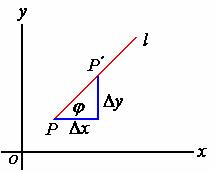
\includegraphics[width=8cm]{image016.jpg}
		\caption{方向导数图示}
	\end{figure}
	\begin{align*}
		\frac{\vartheta f}{\vartheta l} & =\lim_{\rho\to 9}\frac{f(x+\Delta x, y + \Delta y) - f(x,y)}{\rho}                               \\
		                                & =\frac{\vartheta f}{\vartheta x}\cdot\cos\varphi+\frac{\vartheta f}{\vartheta y}\cdot\sin\varphi
	\end{align*}
	函数在点增长最快的方向与方向导数达到最大的方向(梯度方向)是一致的.
	\subsubsection{梯度}
	\begin{gather*}
		gradf(x,y)=\frac{\vartheta f}{\vartheta x}\overrightarrow{i}+\frac{\vartheta f}{\vartheta y}\overrightarrow{j}\\
		\frac{\vartheta f}{\vartheta l}=\left\lvert gradf(x,y)\right\rvert \cdot \cos (gradf(x,y),\overrightarrow{e})
	\end{gather*}
	函数在点P(x,y)增长最快的方向与方向导数达到最大的方向(梯度方向)是一致的.
	\subsubsection{等高线}
	\subsection{多元函数极值}
	定理一:
	设函数在点$(x_0,y_0)$具有偏导数且取极值,则$f_x(x_0,y_0)=f_y(x_0,y_0)=0$\\
	注意:可(偏)导函数的极值点必为驻点,反过来,函数的驻点却不一定是极值点,偏导数不存在的点也可能是极值点
	定理二:对函数z=f(x,y)
	\begin{gather*}
		A=f_xx(x_0,y_0), B=f_xy(x_0,y_0), C=f_yy(x_0,y_0)\\
		\begin{vmatrix}
			A & B \\
			B & C
		\end{vmatrix}=\begin{cases}
			>0\begin{cases}
				  A>0 \Leftrightarrow\text{极小值} \\
				  A<0 \Leftrightarrow\text{极大值}
			  \end{cases} \\
			<0\text{无极值}                    \\
			=0\text{无法判定}
		\end{cases}
	\end{gather*}

	\subsubsection{多元函数最值}
	若z=f(x,y)在\textcolor{blue}{有界区域D上连续}函数最值可能在D内部或边界\\
	最值求法:
	\begin{center}
		1.在D内部使$f_x=f_y=0$或使$f_x,f_y$不存在的点\\
		2.计算所在D内部所疑极值点处函数值\\
		3.求D边界最值\\
		4.比较函数值大小,大者最大值,小者最小值
	\end{center}
	\subsection{开区域D函数最值}
	问题复杂,可根据问题性质断定函数最值在D上取得,而函数在D上恰又只有一个驻点,则该驻点函数值为函数在D上最值
	\subsubsection{条件极值\&拉格朗日乘数法}
	除了函数自变量限制于定义域无其他约束条件$\rightarrow$无条件极值\\
	实际问题:条件极值$\to$无条件极值

	求z=f(x,y)在$\varphi(x,y)=0$线之下极值,若$P_0(x_0,y_0)$处取得,则
	$$
		\begin{cases}
			f_x(x_0,y_0)+\lambda\varphi_x(x_0, y_0)=0 \\
			f_y(x_0,y_0)+\lambda\varphi_y(x_0, y_0)=0 \\
			\varphi(x_0, y_0)=0
		\end{cases}
	$$
	恰是$F(x,y,\lambda)=f(x,y)+\lambda\varphi(x,y)$三个偏导数在点$(x_0, y_0)$处值.

	拉格朗日乘数:作上文拉氏函数,解方程组求出的点(x,y)即是可疑条件极值

	注意:推广至一般元或任意条限制条件$u=f(a_1,a_2, \ldots,a_i)$在限制条件\\$\varphi_1(a_1,a_2, \ldots,a_i)=0, \ldots, \varphi_j(a_1,a_2, \ldots,a_i)=0$
		\begin{align*}
			 & F(a_1,a_2, \ldots,a_i, b_1,b_2, \ldots,b_j)=f(a_1,a_2, \ldots,a_i)+b_1\varphi_1(a_1,a_2, \ldots,a_i)+\ldots+b_j\varphi_j(a_1,a_2, \ldots,a_i) \\
			 & F_{a_1}=0, \ldots, F_{a_i}=0,F_{b_1}=0, \ldots, F_{b_j} = 0
		\end{align*}
		求出$a_1, \ldots, a_i$即是坐标
		\subsection{二重积分}
		\begin{gather*}
			\iint_D f(x,y)d\sigma=\lim_{\lambda\to 0}\sum_{i = 1}^{n} f(\xi_i, \eta_i )\Delta\sigma _i
			\\f(x,y)\text{被积函数}\quad f(x,y)d\sigma\text{被积表达式}\\
			d\sigma\text{面积元素}
		\end{gather*}
		性质:
		1.线性性$\iint_{D}[\alpha\cdot f(x,y)+\beta\cdot g(x,y)]d\sigma = \alpha\cdot\iint{D}f(x,y)d\sigma+\beta\cdot\iint{D}g(x,y)d\sigma
	$\\
		2.区域可加性\\
		3.$f(x,y)\equiv 1 \quad \sigma =\iint_{D}1d\sigma =\iint_{D}d\sigma$
		4.若D存在f(x,y)<$\varphi (x,y)$
	$$\iint_{D}f(x,y)d\sigma \leq \iint_{D}\varphi(x,y)d\sigma$$
	特别地,当$-\lvert f(x,y) \rvert\leq f(x,y)
		\leq \lvert f(x,y) \rvert$
	$$
		\lvert \iint_{D}f(x,y)d\sigma \rvert \leq \iint_{D}\lvert f(x,y)\rvert d\sigma
	$$
	5.估值不等式
	M,m分别为f在D上最大最小值,$\sigma$是M面积,则:
	$$
		m\cdot\sigma \leq \iint_{D}f(x,y)d\sigma \leq M\cdot\sigma
	$$
	6.中值定理
	$\sigma$是D面积,至少一点$(\xi ,\eta)$使
	$$
		\iint_{D}f(x,y)d\sigma=f(\xi ,\eta)\cdot\sigma
	$$

	\subsection{二重积分计算}
	$$
		\iint_{D}f(x,y)d\sigma=\int_{a}^{b}[\int_{\varphi_1(x)}^{\varphi_2(x)}f(x,y)dy]dx
	$$
	称作先对y后对x的二次积分,也可先对x后对y
	\subsubsection{二重积分化二次积分注意}
	对于I型II型用平行于xy轴的直线穿过区域内部与边界交点不多于两点\\
	不满足可对区域进行剖分

	几何法确定定积分的限

	求曲面围成立体的体积\\
	1.先做出立体简图,确定在xoy平面上的投影区域\\
	2.列出体积表达式
	3.配置积分限,化二重积分为二次积分并作定积分计算

	\subsubsection{利用极坐标计算二重积分}
	\begin{align*}
		\Delta\sigma_i & =\frac{\Delta\theta_i}{2}[(r_i+\Delta r_i)^2-r_i^2] \\
		               & =\overline{r_i}\Delta r_i\Delta\theta_i
	\end{align*}
	在$\Delta\sigma_i $取$(\overline{r_i},\overline{\theta_i})$设直角坐标$(\xi_i, \eta_i)$
	\begin{gather*}
		\xi_i=\overline{r_i}\cos\overline{\theta_i}\quad \eta_i=\overline{r_i}\sin\overline{\theta_i}\\
		\iint_{D}f(x,y)dxdy=\iint_{D}f(r\cos\theta, r\sin\theta)rdrd\theta
	\end{gather*}
	二重积分化为极坐标进行运算的关键在于将积分区域D用极坐标表示为$\alpha\leq\theta\leq\beta,\varphi_1(\theta)\leq r \leq\varphi_2(\theta)$

	方式:
	先画区域简图,确定极角最大变化范围$[\alpha,\beta]$\\
	再过$[\alpha,\beta]$内任意一点$\theta$作涉嫌过区域与边界有两交点,用极坐标表示极径变化范围$[\varphi_1(\theta),\varphi_2(\theta)]$
	结论:
	$$
		D:x^2+y^2\leq a^2\quad
		\iint_{D}e^{-x^2-y^2}dxdy=\pi(1-e^{-a^2})
	$$
	著名概率积分:
	$$
		I=\int_{0}^{+\infty}e^{-x^2}dx
	$$
	\begin{figure}[htbp]
		\centering
		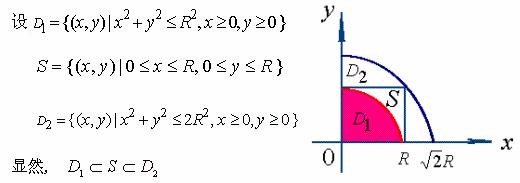
\includegraphics[width=8cm]{image293.jpg}
		\caption{构造概率积分关系}
	\end{figure}
	由$e^{-x^2-y^2}>0$从而
	\begin{gather*}
		\iint_{D_1}e^{-x^2-y^2}dxdy<\iint_{S}e^{-x^2-y^2}dxdy<\iint_{D_2}e^{-x^2-y^2}dxdy\\
		\frac{\pi}{4}\leftarrow^{R\to +\infty}\frac{\pi}{4}(1-e^{-R^2})<(\int_{0}^{R}e^{-x^2}dx)^2<\frac{\pi}{4}(1-e^{-2R^2})\rightarrow^{R\to +\infty}\frac{\pi}{4}\\
		R\to +\infty\quad I=\frac{\sqrt{\pi}}{2}
	\end{gather*}
	原则:
	积分区域边界曲线易于极坐标方程表示(含圆弧,直线段)\\
	被积函数表示式用极坐标变量表示较简单($(x^2+y^2)^a$, a为实数).
	\subsection{三重积分}
	函数在区域连续则三重积分存在
	\begin{align*}
		                  & a\leq x\leq b, y_1(x)\leq y\leq y_2(x), z_1(x)\leq z\leq z_2(x)             \\
		\iiint_{\Omega}dv & =\iint_{D_{xy}}F(x,y)dxdy                                                   \\
		                  & =\int_{a}^{b}dx\int_{y_1(x)}^{y_2(x)}dy\int_{z_1(x,y)}^{z_2(x,y)}f(x,y,z)dz
	\end{align*}
	它将三重积分化成先对积分变量z,次对y,最后对x的三次积分.\\
	如果平行于z轴且穿过$\Omega$内部的直线与边界曲面的交点多于两个,可仿照二重积分计算, 将$\Omega$剖分成若干个部分,化为各部分区域上的三重积分.
	\subsubsection{柱面坐标球面坐标算三重积分}
	点M直角与柱面关系
	$$
		\begin{cases}
			x=r\cos\theta & 0\leq r \leq +\infty        \\
			y=\sin\theta  & 0\leq \theta \leq 2\pi      \\
			z=z           & -\infty\leq z \leq + \infty
		\end{cases}
	$$
	$$
		\iiint_{\Omega}f(x,y,z)dv=\iiint_{\Omega}f(r\cos\theta, r\sin\theta,z)rdrd\theta dz
	$$
	方法:
	1.找出$\Omega$在xoy面上的投影区域$D_{xy}$, 并用极坐标变量$r,\theta$表示之.\\
	2.在内任取一点, 过此点作平行于z轴的直线穿过区域, 此直线与边界曲面$\Omega$的两交点之竖坐标( 将此竖坐标表示成$r,\theta$的函数 )即为z的变化范围.

	点M直角与球面关系
	$$
		\begin{cases}
			x=r\cos\theta & 0\leq r \leq +\infty        \\
			y=\sin\theta  & 0\leq \theta \leq 2\pi      \\
			z=z           & -\infty\leq z \leq + \infty
		\end{cases}
	$$
	$$
		\iiint_{\Omega}f(x,y,z)dv=\iiint_{\Omega}f(r\sin\varphi\cos\theta, r\sin\varphi\sin\theta,r\cos\varphi)r^2\sin\varphi drd\varphi d\theta
	$$
	\subsection{对弧长积分}
	在曲线弧L上对弧长的曲线积分记作:
	$$
		\int_{L}f(x,y)ds
	$$
	注意:
	1.被积函数f(x,y)的定义域为L上一切点\\2.
	2.空间曲线
	$$\int_{\Gamma }f(x,y,z)ds=\lim_{\lambda\to 0}\sum_{i=0}^{n}f(\xi_i,\eta_i,\zeta_i)\cdot\Delta s$$
	3.若L封闭曲线则记作$\oint_L f(x,y)ds$

	性质:1.线性性\\2.$\int_L ds =L$的长度\\3.L上f(x,y)<g(x,y)则$\int_Lf(x,y)ds\leq\int_Lg(x,y)ds$
	\\
	4.$\int_Lf(x,y)ds=\int_{L1}f(x,y)ds+\int_{L2}f(x,y)ds$

	\subsubsection{弧长曲线计算法}
	曲线I由参数方程
	$$
		\begin{cases}
			x=\varphi(t) & \alpha\leq t \leq \beta \\
			y = \phi(t)
		\end{cases}
	$$
	$$
		\int_L f(x,y)ds=\int_{\alpha}^{\beta}f[\varphi(t), \phi(t)]\sqrt{[\varphi^{\prime}(t^2)]+[\phi^{\prime}(t^2)]}dt\quad a\leq \beta
	$$
	由此推出
	$$
		\begin{cases}
			1.y=\phi(x) (a\leq x\leq b) & \int_L f(x,y)ds=\int_{\alpha}^{\beta}f[x, \phi(x)]\sqrt{1+[\phi^{\prime}(t^2)]}dx                                                                       \\
			2.x=\phi(y)                 & \ldots                                                                                                                                                  \\
			3.\begin{cases}
				  x=\varphi(t) \\
				  y=\phi(t)    \\
				  z=\omega(t)
			  \end{cases}             & \int_\Gamma f(x,y,z)ds=\int_{\alpha}^{\beta}f[\varphi(t), \phi(t), \omega(t)]\sqrt{[\varphi^{\prime}(t^2)]+[\phi^{\prime}(t^2)]+[\omega^{\prime}(t^2)]}dt
		\end{cases}
	$$
	\subsubsection{对坐标的曲线积分}
	假定曲面光滑,一般曲面双侧的,法向量指定后为有向曲面.$\Sigma$有向曲面,取一小块曲面$\Delta S$设$\cos\gamma$是$\Delta S$法向量与z轴夹角$\gamma$
	余弦.$(\Delta\sigma)_{xy}$
	$$(\Delta S)_{xy}=\begin{cases}
			(\Delta\sigma)_{xy}  & \cos\gamma > 0      \\
			-(\Delta\sigma)_{xy} & \cos\gamma < 0      \\
			0                    & \cos\gamma \equiv 0
		\end{cases}$$同样有$(\Delta S)_{xz}$,$(\Delta S)_{yz}$

	流向曲面$\Sigma$指定侧流量\begin{align*}
		\Phi & = \lim_{\lambda \to 0}\sum_{i=1}^{n}P(\xi_i ,\eta_i, \zeta_i)(\Delta S_i)_{yz}+Q(\xi_i ,\eta_i, \zeta_i)(\Delta S_i)_{zx}+R(\xi_i ,\eta_i, \zeta_i)(\Delta S_i)_{xy} \\&=\iint_\Sigma P(x,y,z)dydz+Q(x,y,z)dzdx+R(x,y,z)dxdy
	\end{align*}
	性质:1.区域可加性2.取相反侧积分变号$\iint_\Sigma P(x,y,z)dydz=-\iint_{\Sigma^{-}} P(x,y,z)dydz\ldots$

	\begin{align}\label{eq3}
		\iint_\Sigma R(x,y,z)dxdy = \iint_{D_{xy}} R[x,y,z(x,y)]dxdy
	\end{align}
	计算对坐标的曲面积分时,只要把其中变量z换成$\Sigma$方程,然后在的投影区域$D_{xy}$上计算二重积分就成.
	必须注意:公式(3)的曲面积分是取在曲面上侧的;如果曲面积分取在曲面下侧,这时$\cos\gamma < 0$,那末$\iint_\Sigma R(x,y,z)dxdy = -\iint_{D_{xy}} R[x,y,z(x,y)]dxdy$

	右式极限值就叫做函数在有向曲线弧上对x坐标的曲线积分,同理可得y.L为积分弧段.
	$$
		\int_L P(x,y)dx=\lim_{\lambda\to 0}\sum_{i=1}^{n}P(\xi_i, \eta_i)\Delta x_i\quad \int_L Q(x,y)dy=\lim_{\lambda\to 0}\sum_{i=1}^{n}Q(\xi_i, \eta_i)\Delta y_i
	$$
	注意:1.dx为ds在x轴上投影,dx可正可负与恒为正ds区别\\
	2.变力$\overrightarrow{F}(x,y)=P(x,y)\overrightarrow{i}+Q(x,y)\overrightarrow{j}$沿曲线L做功为:$$w=\int_LP(x,y)dx + Q(x,y)dy$$3.推广至空间有向曲线弧$\Gamma$为$$
		\int_\Gamma P(x,y,z)dx=\lim_{\lambda\to 0}\sum_{i=1}^{n}Q(\xi_i, \eta_i, \zeta_i )\Delta x_i\ldots
	$$
	4.坐标曲线积分存在定理,P在L上连续则可对P积分

	性质:1.区域可加性\\2.设$L^{-}$与L方向相反$\int_LPdx + Qdy=-\int_{L^{-}}Pdx + Qdy$3.线性性\\
	\begin{figure}[htbp]
		\centering
		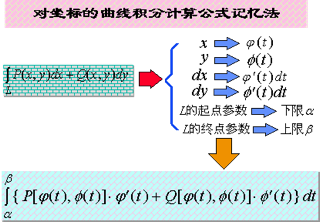
\includegraphics[width=8cm]{image236.png}
		\caption{坐标曲线积分公式记忆}
	\end{figure}
	特殊情形
	$$\int_LP(x,y)dx + Q(x,y)dy=
		\begin{cases}
			\int_{a}^{b}{P[x,\phi(x)], Q[x,\phi(x)]\phi^{\prime}(x)}dx                                                                                                                      & y = \phi(x)    \\
			\ldots                                                                                                                                                                          & x = \varphi(y) \\
			\begin{split}
				\int_{a}^{b}\lbrace P[\varphi(t),\phi(t), \omega(t)]\cdot\varphi^{\prime}(t)+Q[\varphi(t),\phi(t), \omega(t)]\cdot\phi^{\prime}(t)\\
				+R[\varphi(t),\phi(t), \omega(t)]\cdot\omega^{\prime}(t)\rbrace
			\end{split} & \Gamma :x=\varphi(t), y=\phi(t), z=\omega(t)
		\end{cases}
	$$
	一类:两个对坐标的曲线积分尽管被积函数相同,积分曲线的起止相同,积分曲线不同,值不同\\
	虽然沿不同的曲线弧,但第二类曲线积分的值可以是相同的.换句话说,计算曲线积分时, 积分值仅与起点, 终点的坐标有关, 而与连接这两点的曲线形式无关.

	\subsubsection{两类曲线积分关系}
	$$
		\int_LPdx + Qdy=\int_L[P\cos\alpha+Q\cos\beta]ds
	$$
	这里$\alpha=\alpha(x,y), \beta=\beta(x,y)$为有向曲线弧L上点(x,y)处切线向量的方向角

	设$\Sigma$是方程z=z(x,y)给出的曲面上侧,由\eqref{eq3}$\Sigma$方向余弦$$\begin{cases}
			\cos\alpha=\frac{-z_x}{\sqrt{1+z_x^2 + z_y^2}}%TODO
		\end{cases}$$
	得\begin{gather*}
		\iint_\Sigma Pdydz + Qdzdx  +Rdxdy =\iint_\Sigma (P\cos\alpha + Q\cos\beta + R\cos\gamma)dS\\
		\overrightarrow{A} = \lbrace P,Q,R \rbrace\quad \overrightarrow{n}= \lbrace \cos\alpha, \cos\beta, \cos\gamma \rbrace\quad d\overrightarrow{S}=\lbrace dydz, dzdx, dxdy \rbrace\\
		d\overrightarrow{S} = \overrightarrow{n}dS\text{有向面元}\quad \iint_\Sigma \overrightarrow{A}d\overrightarrow{S}=\iint_\Sigma \overrightarrow{A}\overrightarrow{n}dS
	\end{gather*}
	\subsection{格林公式}在平面区域上的二重积分也可以通过沿区域的边界曲线上的曲线积分来表示\\
	单连通区域(D内任一闭曲线所围的部分区域都属于D)复连通区域(含点洞,裂缝)

	区域边界曲线的正向规定:人沿曲线走,区域在左手

	定理:设闭区域D由分段光滑的曲线L围成,函数P(x,y)及Q(x,y)在上D具有一阶连续偏导数,则有$$
		\iint_D(\frac{\vartheta Q}{\vartheta x}-\frac{\vartheta P}{\vartheta y})dxdy=\oint_LPdx+Qdy
	$$
	$$
		A=\frac{1}{2}\oint_L xdy-ydx=\iint_D dxdy
	$$
	注:若区域不满足以上条件,即穿过区域内部且平行于坐标轴的直线与边界曲线的交点超过两点时,可在区域内引进一条或几条辅助曲线把它分划成几个部分区域,使得每个部分区域适合上述条件,仍可证明格林公式成立.\\
	格林公式$\leftrightarrows$二重积分与对坐标的曲线积分
	\subsubsection{平面曲线积分与路径无关的定义}
	开区域,函数一阶连续偏导存在的G内A到B任意两条曲线$L_1,L_2$或任意闭曲线C
	$$
		\begin{cases}
			\int_{L_1}Pdx+Qdy\equiv\int_{L_2}Pdx+Qdy &                 \\
			\oint_LPdx+Qdy=0                         & (L=L_1+L_2^{-}) \\
			\oint_CPdx+Qdy=0                         &
		\end{cases}
	$$
	曲线积分L在G内与路径无关,反之有关

	定理:设开区域G是一个单连通域, 函数P(x,y),Q(x,y)在G内具有一阶连续偏导数,则在G内曲线积分$\int_LPdx+Qdy\Leftrightarrow P_y=Q_x$\\
	使用条件:
	区域G单连通区域\\
	函数P(x,y),Q(x,y)在G内具有一阶连续偏导数
	\subsubsection{对面积曲面积分}
	元素法$$
		\iint_\Sigma f(x,y,z)dS = \lim_{\lambda\to 0}\sum_{i=0}^{n}f(\xi_i,\eta_i,\zeta_i)\cdot\Delta S_i \quad m = \iint_\Sigma \rho (x,y,z)dS$$
	性质:1.存在定理2.曲面可加性3.$\iint_\Sigma dS = \Sigma$4.曲面$\Sigma$上有$f(x,y,z)\leq g(x,y,z)$,则$$
		\iint_\Sigma f(x,y,z)dS \leq \iint_\Sigma g(x,y,z)dS
	$$
	面积积分化二重积分计算$$
		\iint_\Sigma f(x,y,z)dS = \iint_{D_{xy}} f[x,y,z(x,y)]\cdot \sqrt{1+z_x^2(x,y)+z_y^2(x,y)}dxdy
	$$注意:1.被积函数f定义在$\Sigma$上自变量取值满足$\Sigma$方程
	2.同理可求y=(x,y)

	对面积的曲面积分计算的两大要点:
	1、给出曲面$\Sigma$合适的方程形式
	z=(x,y),y=(x,z),x=(y,z)
	2、找出曲面$\Sigma$在相应的坐标面xoy(yoz或xoz)上的投影区域
	$D_{xy}$($D_{yz}$或$D_{xz}$).
	\subsection{高斯公式}
	三重积分与其边界曲面上的曲面积分之间关系.
	定理:设空间闭区域$\Omega $是由分片光滑的闭曲面$\Sigma$所围成,函数P,Q,R在上具有一阶连续偏导数,则有
	\begin{equation}\label{eq4}
		\begin{split}
			\iiint_\Omega (\frac{\vartheta P}{\vartheta x} + \frac{\vartheta Q}{\vartheta y}+\frac{\vartheta R}{\vartheta z})dv &= \oiint_\Sigma Pdydz + Qdzdx + Rdxdy
			\\&= \oiint_\Sigma (P\cos\alpha + Q\cos\beta + R\cos\gamma)dS
		\end{split}
	\end{equation}
	注意:若曲面$\Sigma$不是封闭曲面,不能直接利用高斯公式,需补充曲面

	格林第一公式,其中$\Sigma$是闭区间$\Omega$的整个边界曲面,$\frac{\vartheta v}{\vartheta n}$为函数v沿$\Sigma$的外法线方向的方向导数$$
		\iiint_\Omega u (\frac{\vartheta^2 v}{\vartheta x^2 }+\frac{\vartheta^2 v}{\vartheta y^2 }+\frac{\vartheta^2 v}{\vartheta z^2 })dxdydz = \oiint_\Sigma u \frac{\vartheta v}{\vartheta n }dS - \iiint_\Sigma (\frac{\vartheta u}{\vartheta x} \cdot \frac{\vartheta v}{\vartheta x}+\frac{\vartheta u}{\vartheta y} \cdot\frac{\vartheta v}{\vartheta y}+\frac{\vartheta u}{\vartheta z} \cdot \frac{\vartheta v}{\vartheta z})
	$$

	\emph{
		格林第二公式
		$$
			\iiint_V(u \triangledown ^2 v - v  \triangledown ^2 u)dV = \oiint_S(u \triangledown  v - v  \triangledown  u)d\overrightarrow{S}
		$$
	}

	\subsubsection{沿任意闭曲面的曲面积分为0的条件}
	\begin{figure}[htbp]
		\centering
		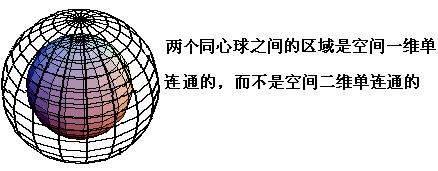
\includegraphics[width=8cm]{image201.jpg}
		\caption{示例}
	\end{figure}
	对空间区G,如果G内任一闭曲面所围成的区域全属于G,则称G是空间二维单连通区域;如果G内任一闭曲线总可以张一片完全属于的曲面,则称G为空间一维单连通区域。

	定理:若在G内曲面积分与所取曲面$\Sigma$无关而只取决于$\Sigma$的边界曲线则:$\iint_\Sigma Pdydz + Qdzdx + Rdxdy\Leftrightarrow\frac{\vartheta P}{\vartheta x}+\frac{\vartheta Q}{\vartheta y}+\frac{\vartheta R}{\vartheta z}=0$

	\subsubsection{通量与散度 高斯公式物理意义}
	设稳定流动的不可压缩液体($\rho = 1$)的速度场:$\overrightarrow{v}(x,y,z)= P(x,y,z)\cdot \overrightarrow{i}+Q(x,y,z)\cdot \overrightarrow{j}+R(x,y,z)\cdot \overrightarrow{k}$则,
	$\Phi = \iint_\Sigma \overrightarrow{v}\overrightarrow{n}\cdot dS$\\如果$\Sigma$是高斯公式\eqref{eq4}中闭区域$\Omega$的边界曲面的外侧
	\begin{figure}[htbp]
		\centering
		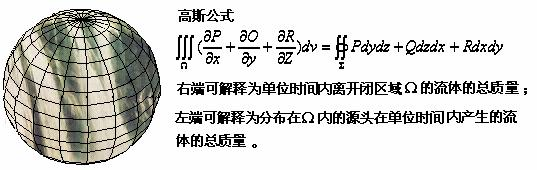
\includegraphics[width=10cm]{image233.jpg}
		\caption{物理意义}
	\end{figure}
	对高斯公式除V应用积分中值定理得:$$\frac{\vartheta P}{\vartheta x} + \frac{\vartheta Q}{\vartheta y} + \frac{\vartheta R}{\vartheta z} = \lim_{\Omega \to M}\frac{1}{M}\oiint_\Sigma v_n dS$$
	左端称为v在点M的散度记作$div v$,在这里可看作稳定流动的不可压缩流体在点的源头强度 — 单位时间单位体积内所产生的流体质量。如果为负,表示点处流体在消失。
	向量场由$\overrightarrow{A}(x,y,z)= P(x,y,z)\cdot \overrightarrow{i}+Q(x,y,z)\cdot \overrightarrow{j}+R(x,y,z)\cdot \overrightarrow{k}$给出,$\oiint_\Sigma \overrightarrow{A}\cdot\overrightarrow{n}dS$叫做向量场通过曲面$\Sigma$向指定侧的通量(流量)$div A = div v$高斯公式可写成$\iiint_\Sigma div A dv = \oiint_\Sigma A_n dS .\quad A_n = \overrightarrow{A}\cdot\overrightarrow{n}=P\cos\alpha + Q\cos \beta + R\cos\gamma$是向量在曲面外侧法向量的投影
	\subsection{斯托克公式}
	斯托克斯公式是格林公式的推广。格林公式表达了平面闭区域上的二重积分与其边界曲线上的曲线积分之间的关系,而斯托克斯公式则把曲面$\Sigma$上的曲面积与沿着$\Sigma$的边界曲线的曲线积分联系起来。
	定理:设$\Gamma$为分段光滑的空间有向闭曲线,$\Sigma$是以$\Gamma$为边界的分片光滑的有向曲面,$\Gamma$的正向与$\Sigma$的侧符合右手规则.

	\begin{equation}\label{斯托克公式}
		\begin{aligned}
			 & \iint_\Sigma (\frac{\vartheta R}{\vartheta y} - \frac{\vartheta Q}{\vartheta z})dydz +(\frac{\vartheta P}{\vartheta z} - \frac{\vartheta R}{\vartheta x})dzdx + (\frac{\vartheta Q}{\vartheta x} - \frac{\vartheta P}{\vartheta y})dxdy=\oint_\Gamma Pdx + Qdy + Rdz=\iint_\Sigma \begin{vmatrix}
				                                                                                                                                                                                                                                                                                     dydz                          & dzdx                          & dxdy                          \\
				                                                                                                                                                                                                                                                                                     \frac{\vartheta}{\vartheta x} & \frac{\vartheta}{\vartheta y} & \frac{\vartheta}{\vartheta z} \\
				                                                                                                                                                                                                                                                                                     P                             & Q                             & R
			                                                                                                                                                                                                                                                                                     \end{vmatrix} \\
			 & (dydz = \cos\alpha, dzdx = \cos\beta, dxdy = \cos\gamma)
		\end{aligned}
	\end{equation}

	如果是面上的一块平面闭区域,斯托克斯公式就变成格林公式。因此,格林公式是斯托克斯公式的一个特殊情形。

	\begin{figure}[htbp]
		\centering
		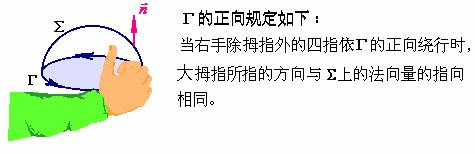
\includegraphics[width=8cm]{image006.jpg}
		\caption{方向规定}
	\end{figure}
	\subsubsection{空间曲线积分与路径无关的条件}
	定理:开空间G一维单连通域,则:
	在G恒成立
	\begin{equation}\label{路径条件1}
		\begin{cases}
			\frac{\vartheta P}{\vartheta y} = \frac{\vartheta Q}{\vartheta x} \\
			\frac{\vartheta Q}{\vartheta z} = \frac{\vartheta R}{\vartheta y} \\
			\frac{\vartheta R}{\vartheta x} = \frac{\vartheta P}{\vartheta z}
		\end{cases}\Rightarrow\int_\Gamma Pdx + Qdy + Rdz\text{空间曲线积分与路径无关}
	\end{equation}

	定理:\eqref{路径条件1}$\Leftrightarrow$表达式$Pdx + Qdy + Rdz$在G内成为函数$u(x,y,z)=\int_{x_0}^{x}P(x,y_0, z_0)dx +\int_{y_0}^{y}P(x,y, z_0)dx + \int_{z_0}^{z}P(x,y, z)dz $的全微分,$M_
		0(x_0, y_0, z_0)\in G$
	\subsubsection{环流量与旋度}
	\begin{gather*}
		\overrightarrow{n}=\cos\alpha\cdot\overrightarrow{i} + \cos\beta\cdot\overrightarrow{j} + \cos\gamma \cdot\overrightarrow{k},\text{有向曲面}\Sigma\text{上(x,y,z)处单位法向量}\\
		\overrightarrow{t}=\cos\lambda\overrightarrow{i}+\cos\mu\overrightarrow{j} + \cos\nu \overrightarrow{k}, \Gamma\text{上(x,y,z)处单位切向量}\\
		\overrightarrow{A}(x,y,z)= P(x,y,z)\cdot \overrightarrow{i}+Q(x,y,z)\cdot \overrightarrow{j}+R(x,y,z)\cdot \overrightarrow{k}\text{在坐标轴上投影的向量叫向量场A的旋度}rot\overrightarrow{A}\\
		\iint_\Sigma rot \overrightarrow{A}\cdot \overrightarrow{n}dS = \oint_\Gamma \overrightarrow{A}\cdot \overrightarrow{t}ds\\
		(rot \overrightarrow{A})_n = (\frac{\vartheta R}{\vartheta y} - \frac{\vartheta Q}{\vartheta z})\cos\alpha +(\frac{\vartheta P}{\vartheta z} - \frac{\vartheta R}{\vartheta x})\cos\beta + (\frac{\vartheta Q}{\vartheta x} - \frac{\vartheta P}{\vartheta y})\cos\gamma \quad\text{A在法向量上的投影}\\
		A_t = P\cos\lambda + Q\cos \mu + R\cos\nu\quad\text{A在切向量上的投影}
	\end{gather*}
	曲线积分$$\eqref{斯托克公式}=\oint_\Gamma (P\cos\lambda + Q\cos \mu + R\cos\nu)ds=\oint_\Gamma A_tds$$
	叫做向量场A沿向闭曲线的环流量\\
	\eqref{斯托克公式}可解释为:向量场A沿有向闭曲线$\Gamma$的环流量等于A的旋度场通过所$\Gamma$张的曲面$\Sigma$的通量,这里$\Gamma$的正向与$\Sigma$的侧应符合右手规则。\\
	旋度来源:旋转角速度与向量场旋度的关系

	\subsubsection{向量微分算子}
	\begin{gather*}
		\triangledown = \frac{\vartheta }{\vartheta x}\overrightarrow{i}+\frac{\vartheta }{\vartheta y}\overrightarrow{j}+\frac{\vartheta }{\vartheta z}\overrightarrow{k}\text{哈密顿算子}\quad
		\triangledown u = \frac{\vartheta u}{\vartheta x}\overrightarrow{i}+\frac{\vartheta u}{\vartheta y}\overrightarrow{j}+\frac{\vartheta u}{\vartheta z}\overrightarrow{k} = grad \  u \quad \triangledown^2 = \triangledown \cdot \triangledown u = \vartriangle u
		\\
		\vartriangle = \frac{\vartheta^2}{\vartheta x^2} + \frac{\vartheta^2}{\vartheta y^2}+\frac{\vartheta^2}{\vartheta z^2}\text{拉普拉斯算子}\\
		\triangledown \cdot \overrightarrow{A} = div A \quad \triangledown \times \overrightarrow{A} = \begin{vmatrix}
			\overrightarrow{i}            & \overrightarrow{j}            & \overrightarrow{k}            \\
			\frac{\vartheta}{\vartheta x} & \frac{\vartheta}{\vartheta y} & \frac{\vartheta}{\vartheta z} \\
			P                             & Q                             & R
		\end{vmatrix} = rot \overrightarrow{A}
	\end{gather*}
	高斯公式斯托克公式表达:$$
		\iiint_\Omega \triangledown \cdot \overrightarrow{A}dv = \oiint_\Sigma A_n dS \quad \iint_\Sigma (\triangledown\times\overrightarrow{A})_n dS = \oint_\Gamma A_t ds
	$$
	\subsection{微分方程}
	解,阶(未知函数最高阶导数),微分方程通解(解含有任意互相独立的常数,👎且其个数与方程的阶数相同),初始条件,特解(确定通解中任意常数),初值问题(满足初始条件的特解)\\一般地讲,微分方程特解的图形是一条曲线,这一曲线称之为积分曲线.
	可化为$g(y)dy = f(x)dx$的是可分离变量微分方程
	设G(x),F(x)分别为g(y),f(x)的原函数,有$G(x)=F(x)+c$(隐式通解)
	通过对微小量的分析得到微分方程.微小量分析法式建立微分方程常用方法.

	\subsubsection{齐次方程}
	若$\frac{dy}{dx}=f(x,y)=\varphi(\frac{y}{x})$,则称齐次方程.引入变量替换$u=\frac{y}{x}, y= u \cdot x$.求出积分后再还原,便得齐次方程的隐式通解.	齐次方程的求解实际上是通过\textcolor{blue}{变量替换将方程化为可分离变量的过程}.
	\subsubsection{一阶线性非齐次方程}
	$$
		\frac{dy}{dx} + P(x)y = Q(x).\begin{cases}
			Q(x) \equiv 0, y = c\cdot e^{-\int P(x)dx + lnc}                                          & \text{齐次}                         \\
			Q(x) \neq 0 ,y = c\cdot e^{-\int P(x)dx}+  e^{-\int P(x)dx}\cdot \int Q(x) e^{P(x) dx}dx, & \text{ 非齐次(常数易变法将c换}u(x))
		\end{cases}
	$$
	一次线性非齐次方程的通解结构=齐次通解+非齐次特解.
	\subsubsection{贝努利方程}
	$$
		\frac{dy}{dx} + P(x) \cdot y = Q(x).\begin{cases}
			n = 0       & \text{一阶线性非齐次}        \\
			n = 1       & \text{一阶线性齐次}          \\
			n \neq 1, 0 & \text{变量代换化为一阶线性}.
		\end{cases}
	$$
	$z = y^{n-1}, \frac{dz}{dx} + (1-n) P(x)\cdot y^{1-n} = (1-n)Q(x)$
	\subsubsection{全微分方程}
	$$
		u=(x,y),du = P(x,y)dx + Q(x,y)dy = 0\quad \text{\OE}
	$$
	因此,若方程Œ的左端是函数的全微分,那么它的通解为u(x,y)=C(任意常数)
	$$\frac{\vartheta P}{\vartheta y} = \frac{\vartheta Q}{\vartheta x} \Leftrightarrow \text{\OE 成为全微分方程}\quad\text{Ž}$$
	\begin{figure}[htbp]
		\centering
		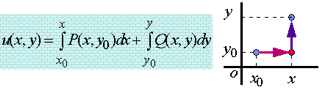
\includegraphics[width=8cm]{image047.png}
		\caption{全微分解法}
	\end{figure}
	Ž不满足时不是微分方程,可找到一个$\mu=\mu(x,y)$乘入使其成立,则称积分因子.
	\subsubsection{可降阶高阶微分方程}
	1.$y^{(n)} = f(x)$.将$y = ^{(n - 1)}$当作新未知函数两边经过n次积分可得含n个任意常数通解.\\
	2.$y^{\prime\prime} = f(x,y^{\prime})$。变量替换$y^{\prime}$化为一阶线性\\
	3.$y^{\prime\prime}=f(y,y^{\prime})$.\\
	注意:求高阶方程满足初始条件的特解时,对应任意常数应及时定出,而不是求出通解后逐一确定,减少计算量
	\subsubsection{高阶线性微分方程}
	有阻尼,物体自由振动的微分方程$\frac{d^2x}{dx^2} + 2n\frac{dx}{dt} + k^2x = 0$.
	若受铅直干扰力$F = H\sin pt$强迫振动的微分方程$\frac{d^2x}{dx^2} + 2n\frac{dx}{dt} + k^2x = h \sin pt, h = \frac{H}{m}$.\\
	一般形式:$\frac{d^2x}{dx^2} + P(x)\frac{dy}{dx} + Q(x)y = f(x), f(x)\equiv 0$则齐次否则非齐次.
	叠加原理:若$,y_1, y_2$为方程两个特解,则$y= c_1y_1 + c_2y_2, c_1,c_2$任意常数也为方程解(非通解).只有当线性无关时才为通解。\\
	设Y为二阶线性齐次的通解,$y^*$为非齐次的特解,则$y = Y + y^*$为二阶线性非齐次方程通解.
	\begin{align*}
		y^{\prime\prime } + P(x)y^{\prime} + Q(x)y & = f_1(x)\text{特解为}y_1^*                        \\
		                                           & = f_2(x)\text{特解为}y_2^*                        \\
		                                           & = f_1(x) + f_2(x)\text{特解为}y^* = y_1^* + y_2^*
	\end{align*}
	可知求特解可以分别求出子表达式的特解然后叠加.
	\subsection{二阶常系数齐次线性微分方程}
	$$
	y^{\prime\prime} + p\cdot y^{\prime} + q\cdot y = 0
	$$
	p,q常数则常系数方程,否则变系数齐次方程.
	r满足特征方程则$y=^{r\cdot x}$为方程的解.
	\begin{figure}[htbp]
		\centering
		\begin{minipage}{0.49\linewidth}
			\centering
			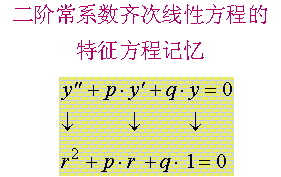
\includegraphics[width=0.6\linewidth]{image032.png}
			\caption{特征方程记忆}
			%\label{chutian1}%文中引用该图片代号
		\end{minipage}
		%\qquad
		\begin{minipage}{0.49\linewidth}
			\centering
			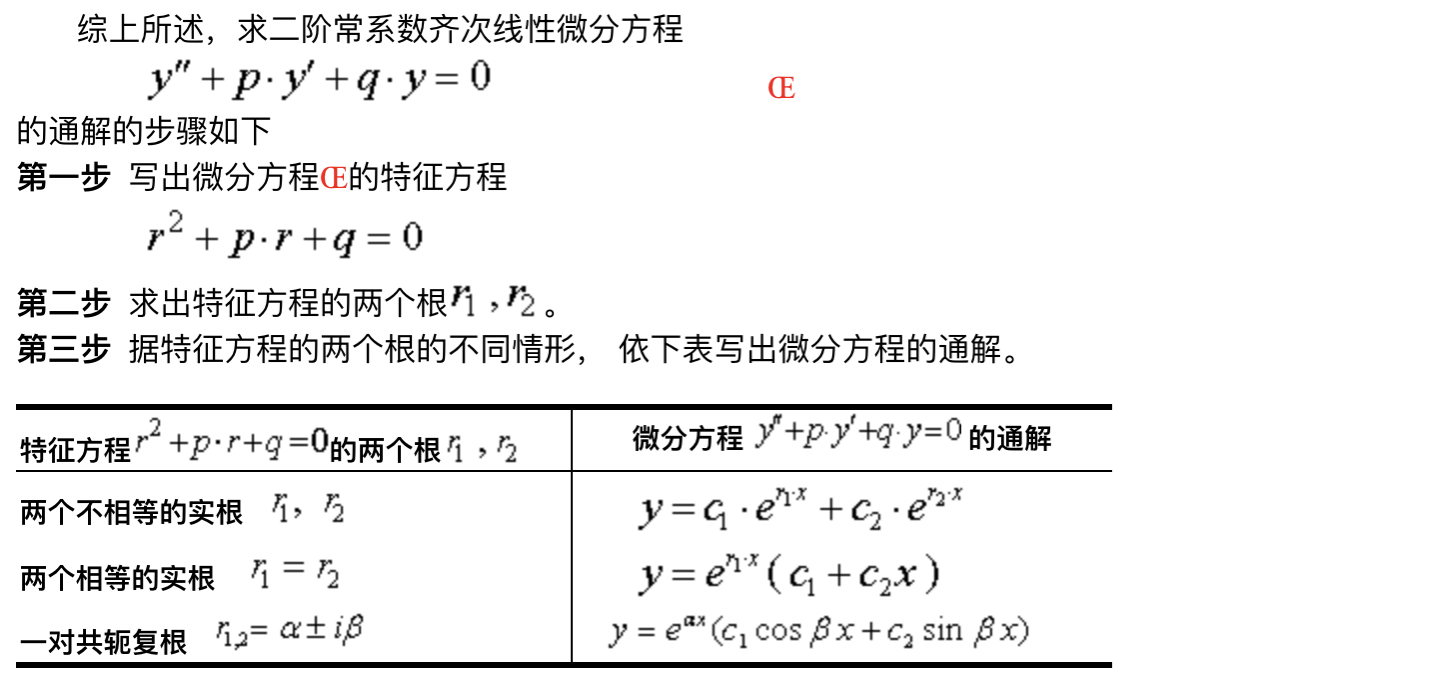
\includegraphics[width=1.5\linewidth]{IMG_5104.jpg}
			\caption{求解}
			%\label{chutian2}%文中引用该图片代号
		\end{minipage}
	\end{figure}
	\subsubsection{n阶常系数齐次线性微分方程}
	\begin{align*}
		&y^{(n)} + p_1 y^{(n-1)} + \ldots + p_n y = 0\\
		&\r^n + + p_1 r^{(n-1)} + \ldots + p_n = 0 
	\end{align*}
	\begin{figure}[htbp]
		\centering
		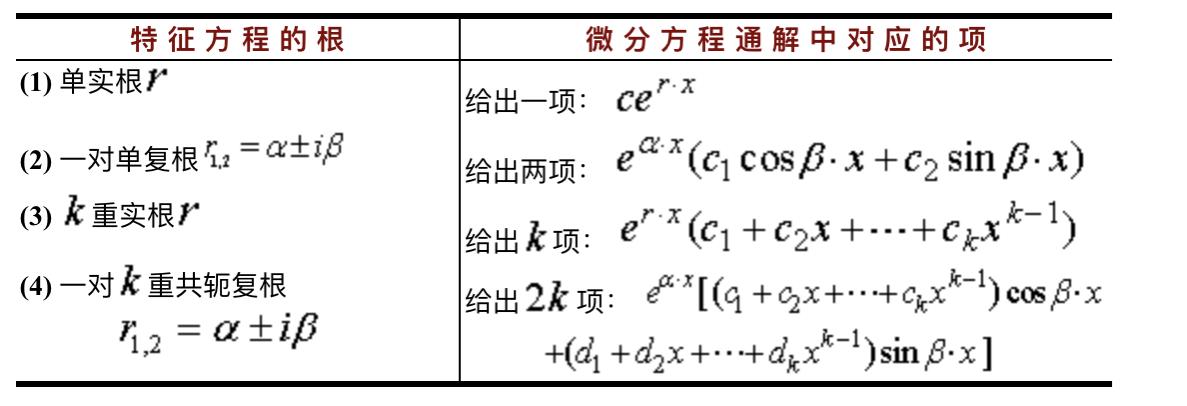
\includegraphics[width=8cm]{IMG_5105.jpg}
		\caption{n阶}
	\end{figure}
\end{sloppypar}
\end{document}